%%%%%%%%%%%%%%%%%%%%%%%%%%%%%%%%%%%%%%%%%
% Short Sectioned Assignment
% LaTeX Template
% Version 1.0 (5/5/12)
%
% This template has been downloaded from:
% http://www.LaTeXTemplates.com
%
% Original author:
% Frits Wenneker (http://www.howtotex.com)
%
% License:
% CC BY-NC-SA 3.0 (http://creativecommons.org/licenses/by-nc-sa/3.0/)
%
%%%%%%%%%%%%%%%%%%%%%%%%%%%%%%%%%%%%%%%%%

%----------------------------------------------------------------------------------------
%	PACKAGES AND OTHER DOCUMENT CONFIGURATIONS
%----------------------------------------------------------------------------------------

\documentclass[paper=a4, fontsize=11pt]{scrartcl} % A4 paper and 11pt font size

\usepackage[T1]{fontenc} % Use 8-bit encoding that has 256 glyphs
\usepackage{fourier} % Use the Adobe Utopia font for the document - comment this line to return to the LaTeX default
\usepackage[english]{babel} % English language/hyphenation
\usepackage{amsmath,amsfonts,amsthm} % Math packages

\usepackage{lipsum} % Used for inserting dummy 'Lorem ipsum' text into the template

\usepackage{sectsty} % Allows customizing section commands
\allsectionsfont{\centering \normalfont\scshape} % Make all sections centered, the default font and small caps

\usepackage{fancyhdr} % Custom headers and footers

% use for graph
\usepackage{graphicx} 
\usepackage{subfigure}
\usepackage{caption}
\usepackage{float} 
\usepackage{url}
\usepackage[colorlinks,linkcolor=blue]{hyperref}
\hypersetup{
    colorlinks=true,
    linkcolor=blue, % 设置链接颜色为蓝色
    urlcolor=blue % 设置网址颜色为蓝色
}

\pagestyle{fancyplain} % Makes all pages in the document conform to the custom headers and footers
\fancyhead{} % No page header - if you want one, create it in the same way as the footers below
\fancyfoot[L]{} % Empty left footer
\fancyfoot[C]{} % Empty center footer
\fancyfoot[R]{\thepage} % Page numbering for right footer
\renewcommand{\headrulewidth}{0pt} % Remove header underlines
\renewcommand{\footrulewidth}{0pt} % Remove footer underlines
\setlength{\headheight}{13.6pt} % Customize the height of the header

\numberwithin{equation}{section} % Number equations within sections (i.e. 1.1, 1.2, 2.1, 2.2 instead of 1, 2, 3, 4)
\numberwithin{figure}{section} % Number figures within sections (i.e. 1.1, 1.2, 2.1, 2.2 instead of 1, 2, 3, 4)
\numberwithin{table}{section} % Number tables within sections (i.e. 1.1, 1.2, 2.1, 2.2 instead of 1, 2, 3, 4)

\setlength\parindent{0pt} % Removes all indentation from paragraphs - comment this line for an assignment with lots of text

%----------------------------------------------------------------------------------------
%	TITLE SECTION
%----------------------------------------------------------------------------------------

\newcommand{\horrule}[1]{\rule{\linewidth}{#1}} % Create horizontal rule command with 1 argument of height

\title{	
\normalfont \normalsize 
\textsc{University College cork} \\ [25pt] % Your university, school and/or department name(s)
\horrule{0.5pt} \\[0.4cm] % Thin top horizontal rule
\huge Modeling Biological Neural Networks \\ % The assignment title
\horrule{2pt} \\[0.5cm] % Thick bottom horizontal rule
}

\author{Kai Deng} % Your name

\date{\normalsize\today} % Today's date or a custom date

% 参考

% https://zhuanlan.zhihu.com/p/66585918
% https://www.jiqizhixin.com/articles/spiking-neurons

\setlength{\abovecaptionskip}{10pt} % 设置图注上方的间隔为5pt
\setlength{\belowcaptionskip}{10pt} % 设置图注下方的间隔为-10pt

\begin{document}
\maketitle % Print the title

\section[short]{Introduction}
\subsection{Background Context}
\subsubsection{Anatomy of a Neuron}
\paragraph{Biological neural networks}
 are complex networks composed of nerve cells (neurons) in organisms (especially human brains and animal brains) and the connections between them. This network is the basis of the biological nervous system and is responsible for processing and transmitting information, allowing organisms to perceive the environment, make decisions, control movement and perform various complex behaviors.

% \begin{figure}[H]
%     \centering
%     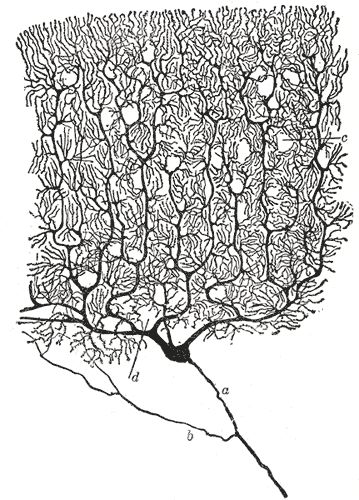
\includegraphics[scale=0.5]{./data/neural-netwrok.jpg}
%     \caption{Human Neural Networks}
%     \label{fig:my_picture}
%     \vspace{6pt} % Vertical space, optional
%     \small{Source: Drawing by the Cajal’s}
% \end{figure}

% \begin{figure}[H]
%     \centering
%     \begin{minipage}[b]{0.45\textwidth}
%         \centering
%         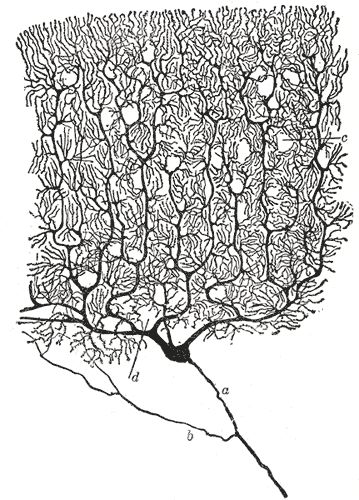
\includegraphics[scale=0.4]{./data/neural-netwrok.jpg}
%         \caption{Human Neural Networks}
%         \label{fig:my_picture}
%         \vspace{1pt} % Vertical space, optional
%         \small{Source: Drawing by the Cajal’s}
%     \end{minipage}
%     \centering
%     \begin{minipage}[b]{0.45\textwidth}
%         \centering
%         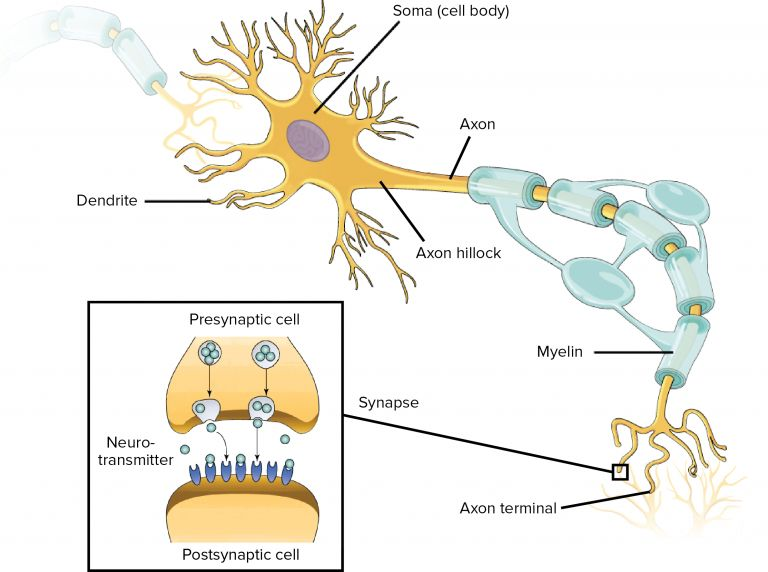
\includegraphics[scale=0.3]{./data/neural.jpg}
%         \caption{Anatomy of the neuron}
%         \label{fig:my_picture}
%         \vspace{1pt} % Vertical space, optional
%         \small{Source: Source:“Neurons and glial cells” by OpenStax College, Biology CC BY-NC-SA 3.0 License.}
%     \end{minipage}
% \end{figure}

\vspace{10pt}
Neurons receive signals from other neurons through synapses located – not exclusively – on their dendritic tree, which is a complex, branching, sprawling structure. If you are wondering what the king of dendritic complexity is, that would be the Purkinje cell, which may receive up to 100,000 other connections. Dendrites are studded with dendritic spines – little bumps where other neurons make contact with the dendrite.

\vspace{10pt}
Signals from the dendrites propagate to and converge at the soma – the cell’s body where nucleus and other typical cell organelles live.

\vspace{10pt}
Coming off the soma is the axon hillock which turns into the axon. The axon meets other neurons at synapses. It allows a neuron to communicate rapidly over long distances without losing signal integrity. To allow signals to travel rapidly, the axon is myelinated – it is covered with interspersed insulators which allows the neuron’s signal to jump between insulated sections. To allow the signal to maintain integrity, the neuron signal in the axon is ‘all-or-nothing’ – it is a rather bit-like impulse, which we will discuss next.


\begin{figure}[H]
    \centering
    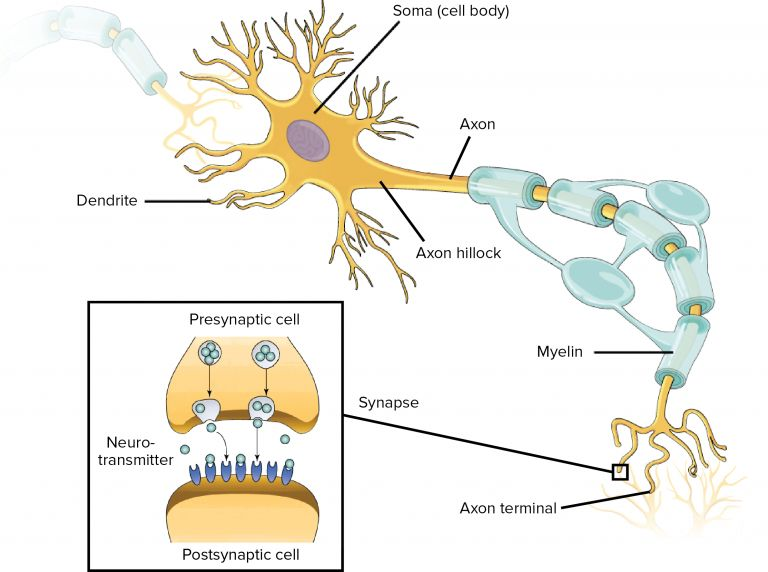
\includegraphics[width=0.9\textwidth]{./data/neural.jpg}
    \caption{Anatomy of the neuron}
    \label{fig:my_picture}
    \vspace{6pt} % Vertical space, optional
    \small{Source: Source:“Neurons and glial cells” by OpenStax College, Biology CC BY-NC-SA 3.0 License.}
\end{figure}


\subsubsection{Physiology of a Neuron}
\paragraph{The}

 second thing to appreciate about neurons is their specialized physiology — that is the cellular functions of neurons. The most striking feature of neural cellular function is the action potential. This is the mechanism which allows neurons to transmit information reliably over long distances without the transmission attenuating.

\vspace{10pt}
It is important to remember that neurons bathe in an extracellular solution of mostly water, salts and proteins. The forces caused by the movement of salts into and out of the cell and the different concentrations of these salts is the physical basis of the neuron’s remarkable behavior. There are sodium-potassium pumps which move sodium out of the cell and potassium in, so that the concentration of sodium outside the cell is higher than inside and the concentration of potassium outside the cell is lower then inside.

\vspace{10pt}
An action potential is a discrete event in which the membrane potential rapidly rises (depolarizes) and then falls (polarizes). This discrete event is all-or-nothing, meaning that if an action potential occurs at one part of the neurons membrane, it will also occur in the neighboring part, and so on until it reaches the axon terminal. Action potentials do not tend to travel backwards, because, once a section of the membrane has fired an action potential, electrochemical-forces hyper-polarize the region of membrane while the channels which were previously open close and become inactive for some duration of time.

\vspace{10pt}
The action potential is the result of different species of ions traveling across the cell membrane through channels and the activation and inactivation of those channels on different time scales. A stereotypical action potential occurs as follows:

\begin{figure}[H]
    \centering
    \begin{minipage}[b]{0.45\textwidth}
      \centering
      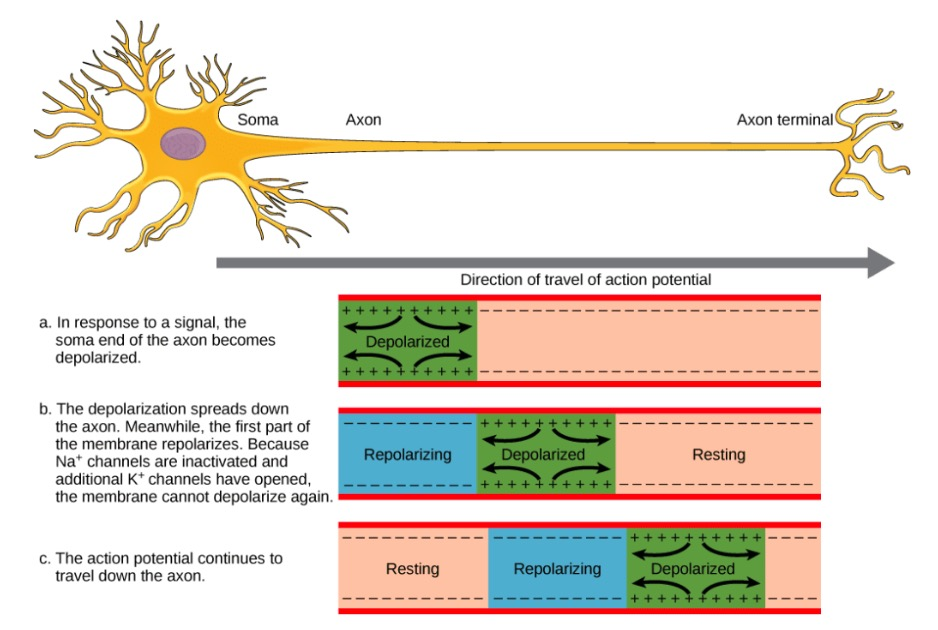
\includegraphics[width=\textwidth]{./data/propagation-of-nerve-impluse.jpg}
      \caption{Propagation of nerve impluse}
      \label{fig:exampleA}
      \vspace{6pt} % Vertical space, optional
      \small{Source: \href{https://opentextbc.ca/biology/chapter/16-2-how-neurons-communicate/}{Opentex}}
    \end{minipage}
    \hfill
    \begin{minipage}[b]{0.45\textwidth}
      \centering
      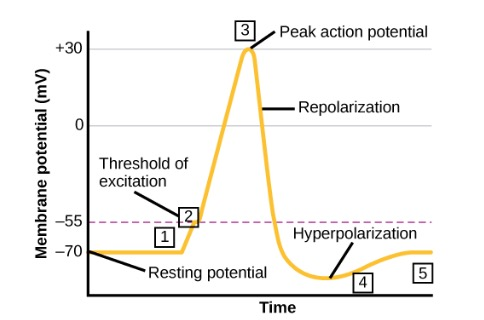
\includegraphics[width=\textwidth]{./data/neuronal-action-potential.jpg}
      \caption{Neuronal action potential}
      \label{fig:exampleB}
      \vspace{6pt} % Vertical space, optional
      \small{Source: \href{https://opentextbc.ca/biology/chapter/16-2-how-neurons-communicate/}{Opentex}}
    \end{minipage}
\end{figure}



\begin{itemize}
    \item \textbf{Equilibrium:} The neuron’s equilibrium membrane potential is near \(-70\) mV — roughly the Nernst Equilibrium of \( E_{K^+} \approx -75 \). At equilibrium, the net current is \(0\) — inward and outward currents are balanced.
    \item \textbf{Depolarization:} Incoming excitatory signals depolarize the membrane. Quick-to-respond voltage gated \( Na^+ \) channels are activated, and \( Na^+ \) rushes in, pushing the membrane potential higher. Slower-to-respond \( K^+ \) channels open, and \( K^+ \) rushes out, pushing the membrane potential lower.
    \item \textbf{Amplification:} If the neuron becomes more stimulated or is stimulated rapidly, many more \( Na^+ \) channels are activated than \( K^+ \) channels. This causes a feedback loop where the influx of \( Na^+ \) causes more \( Na^+ \) channels to activate.
    \item \textbf{Repolarization:} Eventually the membrane potential is near the Nernst Equilibrium of \( Na^+ \) as the sodium channels are maximally open. The slower \( K^+ \) channels catch up to \( Na^+ \), which repolarizes the membrane potential. Meanwhile, the \( Na^+ \) channels become inactive.
    \item \textbf{Hyper-polarization:} \( K^+ \) channels are open while \( Na^+ \) channels are inactive, causing the membrane potential to dip below its typical equilibrium point, near the \( K^+ \) Nernst equilibrium.
    \item \textbf{Refractory Period:} The \( Na^+ \) channels, take a while to become deinactivated, meaning after an action potential, they remain incapable of opening again for a period of time. The period in which most \( Na^+ \) channels are called the absolute refractory period (the neuron cannot spike no matter the strength of the stimulus) while the period in which many \( Na^+ \) channels are inactivated is called the relative refractory period (the neuron can spike given a sufficiently strong stimulus).
\end{itemize}



\subsubsection{Spike train}

Spike trains are the language of neurons. People tend to think of spikes as point-events and spike trains as point-processe. We describe these with the neural response function:

\begin{equation}
    \rho(t) = \sum_{i=1}^{k} \delta(t-t_i)
\end{equation}

where an impulse is defined as the dirac delta function (which is convenient for counting things):

\begin{equation}
    \delta(t) = \begin{cases} 1 & \text{if } t = 0, \\ 0 & \text{otherwise} \end{cases}
\end{equation}

Often, it is useful for analysis to assume spike trains are generated by random processes. Assuming spikes are independent of each other, we can model this point process is a Poisson process, in which we know the probability n spikes occur in the interval $\Delta T$:

\begin{equation}
    P\{n \text{ spikes occur in } \Delta t\} = \frac{(rt)^n}{n!} \exp(-rt)
\end{equation}

To generate spikes according to a Poisson point process, generate a random number 
r
 in a sufficiently small time interval, such that only 1 spike should occur, and check whethe $r < firingRate \Delta T$. However, make sure that $firingRate\Delta T < 1$.


\subsection{Significance of Modeling}
Modeling serves as a pivotal tool in neuroscience, providing insight into the functionality of the brain and the intricate mechanisms of neural processes. It offers a window into the otherwise inaccessible workings of neural communications.

\subsection{Historical Overview}
The endeavor to model neural networks is not new. Groundbreaking models such as the Hodgkin-Huxley and FitzHugh-Nagumo models have been instrumental in advancing our understanding of neural behavior and have set the stage for modern developments in neural modeling.









\subsection{Challenges and Limitations}
Accurately modeling biological neural networks presents numerous challenges. These include the complexity of neuronal dynamics, the nonlinear nature of neural responses, and the vast interconnectivity within the neural network.

\subsection{Recent Advances}
Recent advancements in computational power and mathematical methodologies have allowed for the creation of more sophisticated and detailed models of neural networks, pushing the boundaries of what was previously possible.

\subsection{Applications}
The application of neural network models is vast, ranging from the exploration of neurological disorders, such as epilepsy and Alzheimer’s disease, to the investigation of cognitive processes.

\subsection{Objectives of Your Work}
The objectives of the presented work are to \ldots (here, you would specify the goals of your own research or modeling approach).


% 人类通过研究碳基生物制造硅基生物



%----------------------------------------------------------------------------------------

\bibliographystyle{unsrt} % This specifies the style of the bibliography
\bibliography{/Users/dengkai/workspace/papers/latex/config/ref} % This should match the name of your .bib file without the extension
\end{document}

